\subsection{Organization chart orientation
\label{org-chart-orientation}}

How an organization's culture is conveyed by artifacts like org charts is subtle and can be overanalyzed. 

A common method of describing relations within the bureaucracy is the organization chart (colloquially, the ``org chart"). Normally the CEO is at the top of the chart, middle management is in the middle, and managed employees are at the bottom. See Fig.~\ref{org_chart_orientation_ceo-at-top} 

% What's the point of this section? Is there a consequence, or is this just an observation?
There are emotional connotations to alternative layouts. Convey culture by playing with orientation of the relations.

\begin{itemize}
\item CEO at the bottom -- Fig.~\ref{org_chart_orientation_ceo-at-bottom}
\item CEO on the left -- Fig.~\ref{org_chart_orientation_ceo-follows}
\item CEO on the right -- Fig.~\ref{org_chart_orientation_ceo-leads}
\item CEO as the center of a star\footnote{Example: \href{https://en.wikipedia.org/wiki/File:League_of_Nations_Organization.png}{League of Nations diagram}}
\end{itemize}


\begin{figure}
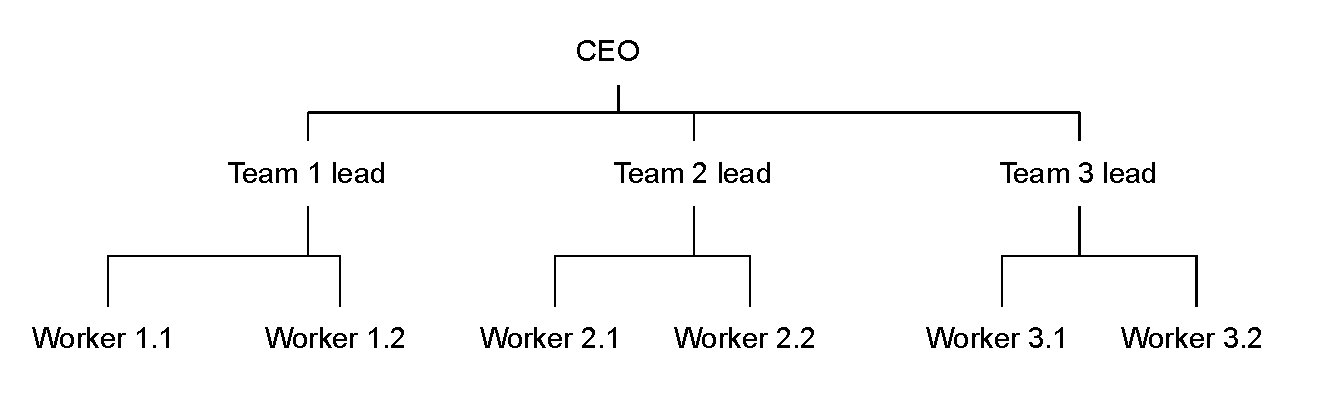
\includegraphics[width=1\textwidth]{images/org-chart-orientation-ceo-at-top.pdf}
\caption{Standard orientation. Role with most responsibility is at top. Left-right ordering is intended irrelevant in this view.}
\label{org_chart_orientation_ceo-at-top}
\end{figure}

\begin{figure}
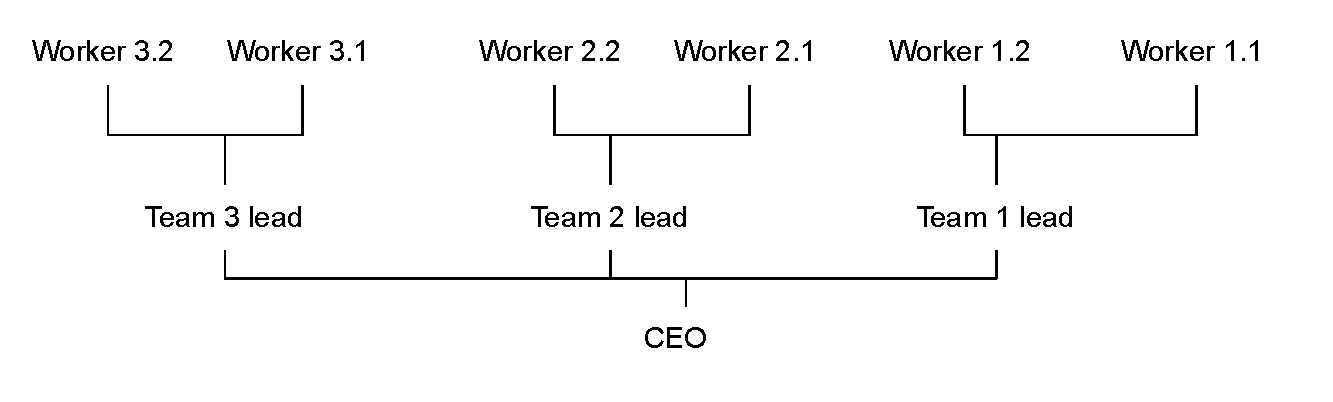
\includegraphics[width=1\textwidth]{images/org-chart-orientation-ceo-at-bottom.pdf}
\caption{Flipping the orientation presents a more realistic burden on the CEO's responsibility. Left-right ordering is intended to be irrelevant in this view.}
\label{org_chart_orientation_ceo-at-bottom}
\end{figure}

\begin{figure}
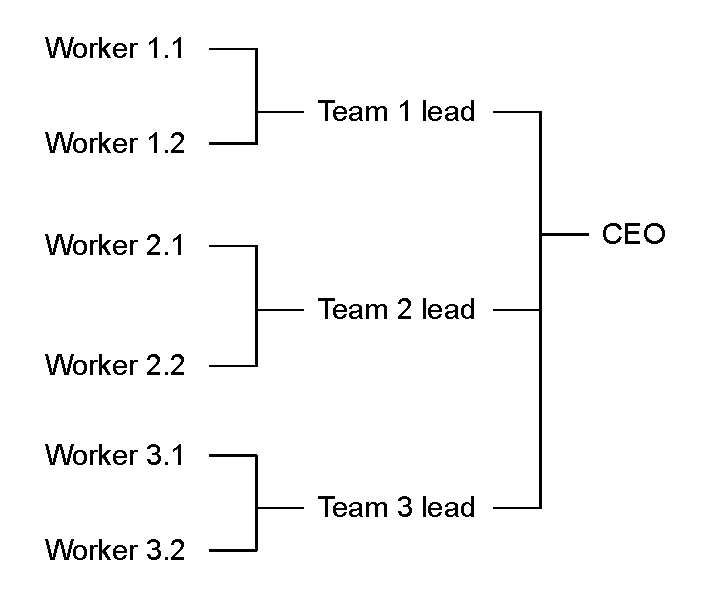
\includegraphics[width=0.8\textwidth]{images/org-chart-orientation-ceo-leads.pdf}
\caption{Conventionally time flows from left (old) to right (new), so in this graph the CEO leads the charge into the unknown. The top-to-bottom ordering can be read as importance. }
\label{org_chart_orientation_ceo-leads}
\end{figure}

\begin{figure}
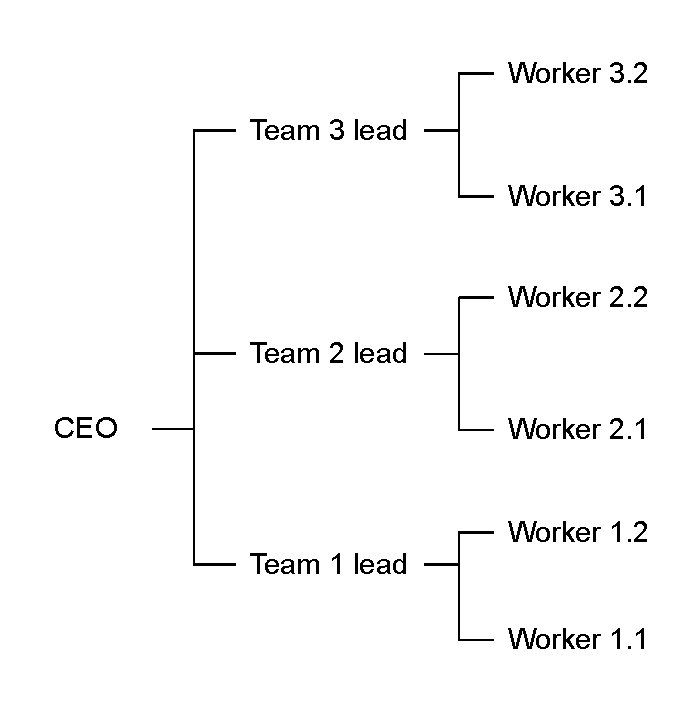
\includegraphics[width=0.8\textwidth]{images/org-chart-orientation-workers-lead.pdf}
\caption{The ``chariot view'' with the CEO in the chariot and the workers out front. As with Fig.~\ref{org_chart_orientation_ceo-leads}, top-to-bottom ordering can be read as importance. }
\label{org_chart_orientation_ceo-follows}
\end{figure}
